\chapter{The Braid Group}
\label{ch:braid_group}

\begin{definition}
    The \textit{configuration space} of $n$ ordered distinct points in the complex plane $\C$ is defined as $M_n = \left\{ \left( z_1,\dots,z_n \right)\in\C ; z_i\neq z_j,\forall i\neq j \right\}$. Alternatively, consider $\mathcal{D}$ to be the collection of all hyperplanes $H_{i,j}=\left\{ z_i=z_j \right\}\in\C^n$ for $1\leq i < j \leq n$. Then we can define $M_n = \C^n \setminus \mathcal{D}$.
\end{definition}

Note that $\left( z_1,z_2,z_3,\dots,z_n \right)$ and $\left( z_2,z_1,z_3,\dots,z_n \right)$ are different points in the configuration space $M_n$. Before studying the various interpretations of the braid group, we first define the braid group itself.

\begin{definition}
    The \textit{pure braid group} on $n$ strands, denoted $PB_n$, is the fundamental group of $M_n$. One can write $PB_n = \pi_1(M_n)$.
\end{definition}

\section{Visualization of pure braids}

We can think of a pure braid as a loop in $M_n$:
\begin{align*}
    \beta : \left[ 0,1 \right] &\to M_n \\
    t &\mapsto \beta(t) = \left( \beta_1(t),\beta_2(t),\dots,\beta_n(t) \right),
\end{align*}
with some base point. Conventionally, we define the base point as the $n$-tuple of integers $(1,2,3,\dots,n)\in \C^n$. Then a pure braid can be though of the motion of these points in the complex plane as $t$ ranges from 0 to 1 in which $\beta_i(t)$ is defined and $\beta_i(t)\neq \beta_j(t)$ for every $t\in[0,1]$ and $i\neq j\in\left\{ 1,2,\dots,n \right\}$. Because each $\beta_i$ is a loop, it must start and end at the point $i$ (e.g., $\beta_i(0)=\beta_i(1)=i$). Recall that the loops are actually equivalence classes of loops under homotopy. As a result, we can continuously deform the motion of the $n$ points while maintaining the same pure braid (up to equivalence) so long as we preserve the pairwise distinction of the points for all time $t\in[0,1]$.

A common visualization of pure braids is to plot the motion of the points in 3-dimensional space. For each $t\in [0,1]$, we draw the points $\left( \beta_i(t),t \right)$ in $\C\times[0,1]$ for every $i\in\left\{ 1,\dots,n \right\}$. The space $\C\times[0,1]$ can be thought of as a spacetime diagram, where the motion of the points is plotted in the complex plane at each time $t$, with the time being the vertical axis. The convention is to have $\C\times\left\{ 0 \right\}$ placed above $\C\times\left\{ 1 \right\}$, so that the motion of the points is plotted from top to bottom.

For every $i\in\left\{ 1,\dots,n \right\}$, the motion of a single point starting at $(i,0)$ and ending at $(i,1)$ is known as the $i$-th \textit{strand} of the pure braid. This can also be described by the $i$-th projection of the $n$-tuple $\beta(t)$. Thus, two braids are equivalent under homotopy if, for every moment of a continuous deformation of the $n$ strands in $\C\times [0,1]$, the (fixed) endpoints $((1,0),(2,0),\dots,(n,0))$ and $((1,1),(2,1),\dots,(n,1))$ are connected by strands that are pairwise disjoint where each strand intersects the plane $\C\times\left\{ t \right\}$ exactly once for every $t\in[0,1]$.

As pure braids are members of the pure braid group, multiplication is a well-defined operation. In the context of $M_n$, multiplication of pure braids involves the concatenation of loops. Visually, this is the process of stacking braids on top of each other, and then rescaling the time dimension so that $t$ ranges from 0 to 1.

\section{General braids}
In the previous section, we defined pure braids in which the endpoints of each strand are identical at the beginning and end of the motion. This notion generalizes to define (non-pure) braids. First, we define a more general configuration space than $M_n$. The symmetric group $S_n$ permutes the $n$ distinct points in $\C$. Then the \textit{configuration space of n unordered points in $\C$} is the quotient space $N_n = M_n/S_n$.

\begin{definition}
    The braid group on $n$ strands is the fundamental group of $N_n$, denoted $B_n = \pi_1(N_n)$.
\end{definition}

The visualization of a braid is the same as in the case of pure braids, only now the endpoints of each strand do not necessarily match the starting points. For example, the $i$-th strand may start at the point $(i,0)$ but end at the point $(j,1)$ for $i,j\in\left\{ 1,\dots,n \right\}$. The equivalence of strands is still defined as before under the homotopy of loops. Loop concatenation defines the multiplication of braids, as before.

\section{Standard generators of the braid group}\label{sec:std_gens}
Originally proposed by Artin~\cite{Artin1947}, each braid can be decomposed into a product of \textit{standard generators} of the braid group. When visualizing braids in $\R\times[0,1]$, a crossing of two strands is clearly indicated by one going over the other. Suppose each crossing occurs at a different time $t\in[0,1]$. Then by rescaling the time component of an arbitrary braid, we can deconstruct it into a stack of simple braids with only one crossing between neighboring strands per braid. Each single crossing of strands can be obtained by performing a transposition between neighboring endpoints of the strands.

For instance, swapping the endpoints of the $i$-th and $(i+1)$-th strands can be written as applying $\sigma_i$ to the identity braid (i.e., the braid that starts without any crossings of strands). It must be noted that there are two distinct ways to swap the endpoints of two strands. From a bottom-up perspective looking at just $\C\times\left\{ 1 \right\}$, $\sigma_i$ swaps $(i,1)$ and $(i+1,1)$ in a counterclockwise rotation. The reverse of this operation (i.e., twisting the endpoints around in the clockwise direction) is denoted $\sigma_i^{-1}$. The standard generators of the braid group $B_n$ are defined as the set $\left\{ \sigma_1,\sigma_2,\dots,\sigma_{n-1} \right\}$. An arbitrary braid can be constructed by concatenating (or stacking) the simple braids made from the standard generators before rescaling the time coordinate to $[0,1]$.

\section{Automorphisms of the free group}

Consider the $n$-times punctured disk $\D_n$. The fundamental group of $\D_n$ involves loops that start and end at the same (fixed) base point in $\partial\D_n$. Up to homotopy, a clockwise loop that only encompasses the $i$-th hole in $\D_n$ is analogous to the $i$-th generator of the free group $F_n$ of rank $n$. In fact, we have $\pi_1\left( \D_n \right) = F_n$. This equality allows us to define a representation of the braid group on $n$ strands as automorphisms of $F_n$.

Each braid $\beta\in B_n$ is realized as an automorphism of $\pi_1(\D_n) = F_n$ (up to isotopy) in which each loop $\gamma\in\pi_1(\D_n)$ is sent to another loop $\beta(\gamma)$. In other words, we have a representation of the braid group defined by
\begin{align}
    \rho: B_n &\to \aut{F_n} \\
    \beta &\mapsto \rho_\beta.
\end{align}
The action of $\beta$ on a loop $\gamma$ is defined by the rearrangements of the $n$ holes in $\D_n$, similar to the action of the standard generators of $B_n$ on the base points in $\C\times\left\{ 1 \right\}$. In terms of the standard generators of $B_n$, each $\sigma_i$ corresponds to switching the places of hole $i$ and hole $i+1$ by means of a counterclockwise rotation, as seen in Figure~\ref{fig:sigma_on_Dn}. This is identical to viewing the action of $\sigma_i$ on the base points in $\C\times\left\{ 1 \right\}$ from the bottom-up, as described in Section~\ref{sec:std_gens}. As before, the inverse action $\iv{\sigma_i}$ is a clockwise rotation of the two adjacent holes $i$ and $i+1$ in $\D_n$. These actions respect the group operation of loop concatenation.

\begin{figure}[htbp]
    \centering
    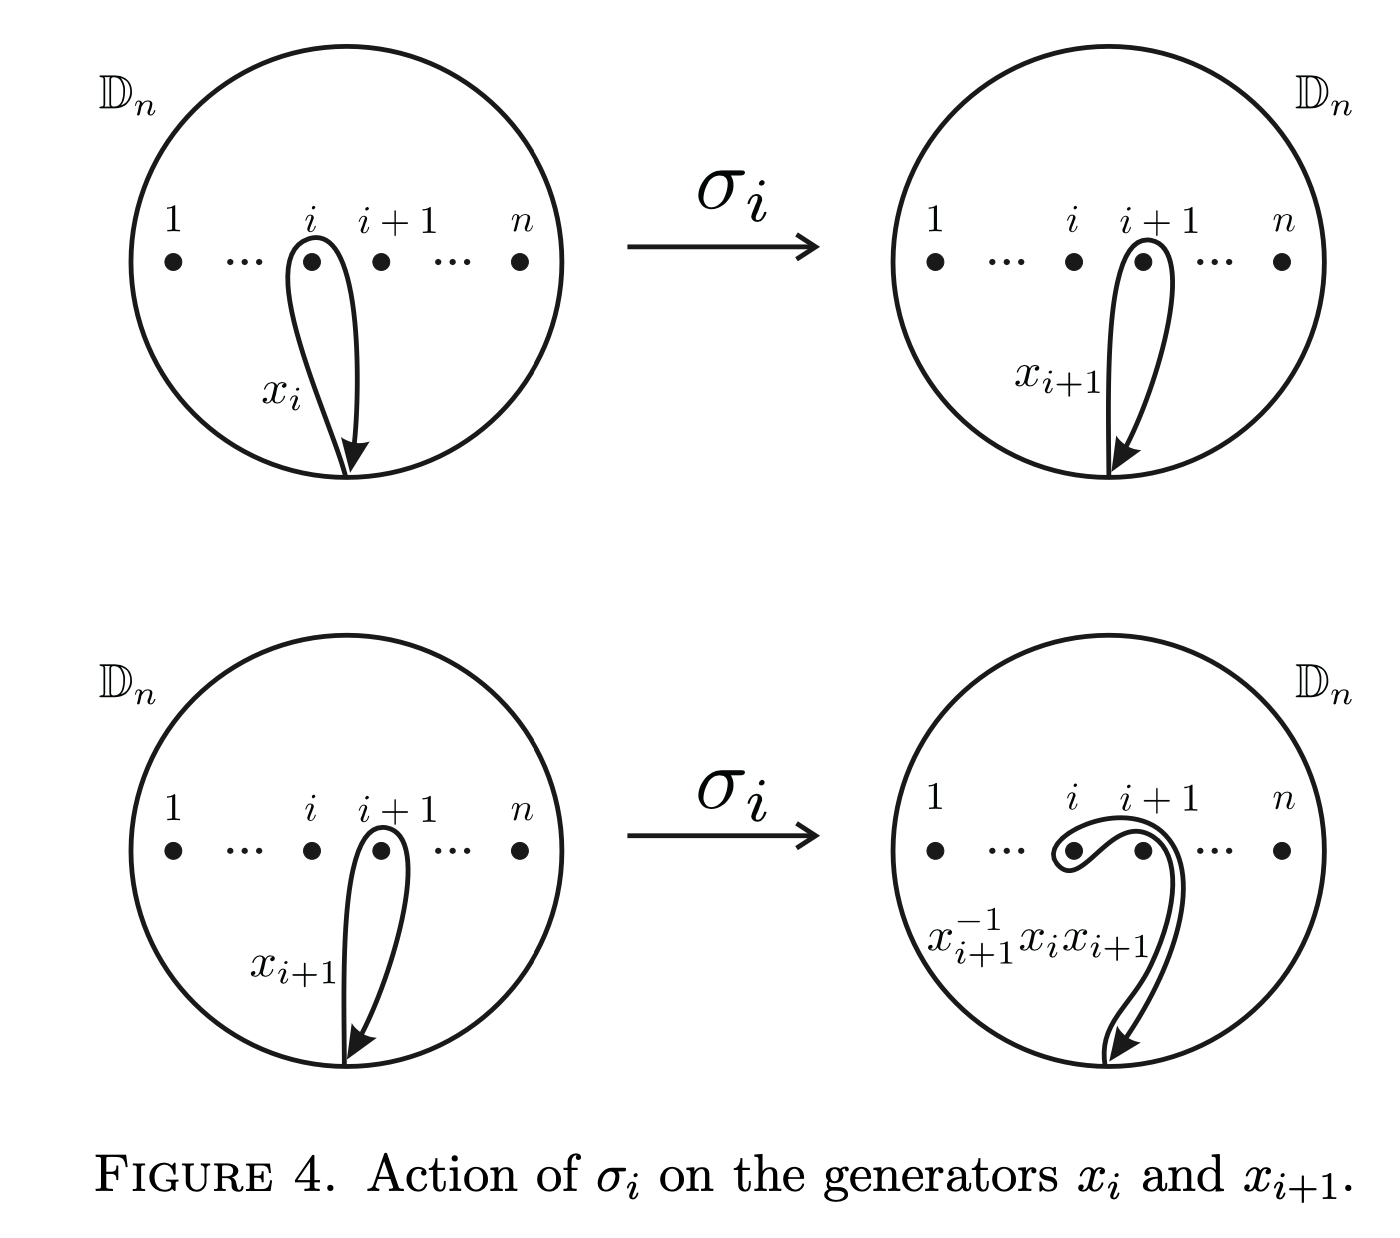
\includegraphics[width = .5\textwidth]{Gonzalez_Fig4_sigma_on_Dn.png}
    \caption{\colorbox{red}{Replace}}\label{fig:sigma_on_Dn}
\end{figure}

The automorphism $\rho_\beta$ is most simply defined in terms of the action of the standard generators of $B_n$ on the generators $x_1,\dots,x_n$ of $F_n$ (visualized as loops in $\D_n$). For each $i\in\left\{ 1,\dots,n-1 \right\}$, it follows that
\begin{align}
    &\rho_{\sigma_i}(x_i) = x_{i+1}, \\
    &\rho_{\sigma_i}(x_{i+1}) = \iv{x_{i+1}}x_i x_{i+1}, \\
    &\rho_{\sigma_i}(x_j) = x_j, \textrm{ for } j\neq i,i+1.
\end{align}
These relations can be verified graphically as in Figure~\ref{fig:sigma_on_x_i}.
\begin{figure}[htbp]
    \centering
    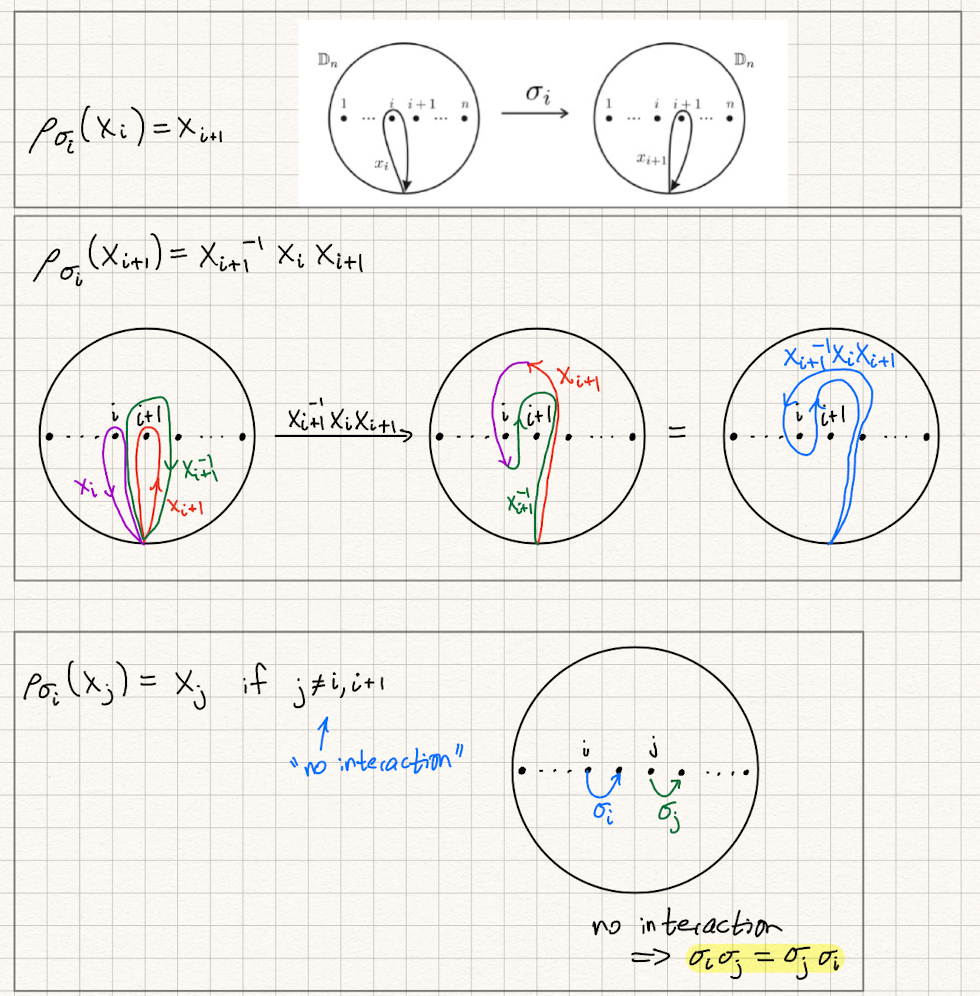
\includegraphics[width = .5\textwidth]{sketch_sigma_on_x_i.png}
    \caption{\colorbox{red}{CAPTION}}\label{fig:sigma_on_x_i}
\end{figure}
For any $\sigma_i$, $\rho_{\iv{\sigma_i}}$ is clearly defined. It follows that for any braid $\beta\in B_n$, we can decompose $\rho_\beta$ the composition of the automorphisms of the standard generators $\sigma_1,\dots,\sigma_{n-1}$ and their inverses that make up $\beta$. 

Notice that for any $\sigma_i$, $\rho_{\sigma_i}(x_1\cdots x_n) = x_1\cdots x_n$. This is because the loop $x_1\cdots x_n$ in $\D_n$, encompassing all holes, is parallel to the boundary $\partial\D_n$. Thus, the action of $\sigma_i$ on $x_1\cdots x_n$ is trivial does not affect the structure of the loop up to isotopy. More generally, this implies that $\rho_\beta(x_1\cdots x_n) = x_1\cdots x_n$ for any $\beta\in B_n$. Paired with the observation that every generator is conjugate to another, Artin~\cite{Artin1947} showed that this is a necessary and sufficient condition for $\rho_\beta$ to be an automorphism of $F_n$.

\begin{theorem}
    An automorphism $f\in\aut{F_n}$ is equal to $\rho_\beta$ for some $\beta\in B_n$ if and only if
    \begin{enumerate}
        \item $f(x_i)$ is a conjugate of some $x_j$ for every $i\in\left\{ 1,\dots,n \right\}$, and
        \item $f(x_1\cdots x_n) = x_1\cdots x_n$.
    \end{enumerate}
\end{theorem}

In this interpretation of the braid group, we can express $B_n$ in terms of the standard generators:
\begin{equation}
    B_n = \left\langle \sigma_1,\dots,\sigma_{n-1} \;\middle|\;
    \begin{aligned}
        \sigma_i\sigma_j &= \sigma_j\sigma_i, & |i-j|&>1 \\
        \sigma_i\sigma_{i+1}\sigma_i &= \sigma_{i+1}\sigma_i\sigma_{i+1}, & |i-j|&=1
    \end{aligned}
    \right\rangle.
\end{equation}
The first condition that the standard generators commute if $|i-j|>1$ is easily verified by looking at the graphic of Figure~\ref{fig:sigma_on_x_i} in describing the property of the automorphism $\rho_{\sigma_i}(\sigma_j) = \sigma_j$. This follows by the fact that if two holes are non-adjacent, then the actions of $\sigma_i$ and $\sigma_j$ are mutually exclusive and thus commutative. The second condition on the standard generators is most easily verified in Figure~\ref{fig:YB_criterion_verification} by looking at the corresponding braids in $\R\times[0,1]$.
\begin{figure}[htbp]
    \centering
    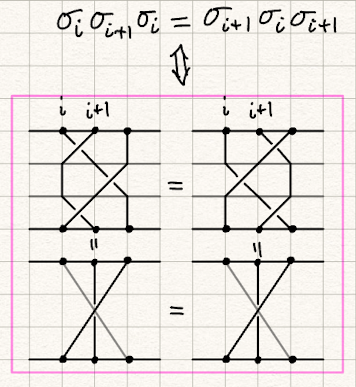
\includegraphics[width = .5\textwidth]{sketch_YB_citerion_verification.png}
    \caption{\colorbox{red}{Grayed-out strand indicates that it is behind all other strands.}}\label{fig:YB_criterion_verification}
\end{figure}